\chapter{Method}

This chapter describes the methods used when implementing the algorithms used to solve the problem, and the evaluation of the outcome.

\section{Considered methods}
TODO! Is this section relevant? % TODO
Object detection: \\
Approxpolydp approach\\
considered efficient line to polygon detection algorithm such as in \cite{joaquim2003polygon}.
However, this method assumes too much about the data to be feasible. Demands too perfect input.

\section{Implementation}
This section presents the methods used when implementing the algorithms used to solve the problem. % Todo rephrase

\subsection{OpenCV} % TODO rephrase
The most important piece of software used in this thesis is the library OpenCV.
It is used extensively in this thesis, and therefore deserves an introduction.

OpenCV is an open source library for computer vision. % footnote to opencv homepage?
It contains functions for many things that one needs when working with computer vision-related fields, from low-level processing such as filters, to high-level functions for feature detection, machine learning, camera calibration, pose estimation, and much more.
It was designed with a strong focus on efficiency to be useful for real-time applications. \cite{bradski2008learning}

OpenCV is written in C and C++, but also has full interfaces for python, java and MATLAB\cite{wiki:OpenCV}.
The native C++ interface was used in this thesis. % Todo tense?

\subsection{Preprocessing}

Preprocessing is the first step in most computer vision algorithms, and can have many purposes. 
In this case, the purpose is to reduce noise, and to remove irrelevant information from the image.
This is accomplished by converting the colour image to a grayscale image, followed by applying a median filter. 
A median filter was chosen because it reduces noise effectively, while also removing small, unwanted features from the image, such as small labels and marks on the package or the rest of the scene.
At the same time edges are preserved.
As the name implies, the median filter assigns the value of every pixel to the median of itself, and the neighbouring pixels within a certain radius. % is this theory?

\subsection{Edge and Line Detection} % TODO bad quality text
The next step is to detect edges in the image, which is done using Canny's edge detection algorithm \cite{canny}.
The output of Canny's Edge detection algorithm is a binary image in which pixels that are considered to be part of an edge are 1 and other pixels are 0.
Now, the information in the edge image needs to be converted to a symbolic format.
To accomplish this, contour analysis is first applied to the binary image using \cite{suzuki}.
The result of the contour analysis is then fed to a line detection algorithm after some pruning.
For this purpose, a line detection algorithm based on a probabilistic version of the hough transform is used \cite{houghp}.
This function outputs a more easy to use format, namely the coordinates of the end points of each detected line.

\subsection{Package Detection}

The algorithm used to detect the package is based on a ranking scheme, where multiple hypothesis about where the package is are created, and then scored. 
The candidate with the highest score is chosen as the package. 

A fundamental property of cuboids is exploited by the algorithm: they consist of parallel line segments of equal length. 
More specifically, the outline of a cuboid in a two dimensional image is made up of three pairs of parallel line segments, which form a hexagon. 
However because of perspective distortion the line segments will not be entirely parallel, and not  of exactly equal length.
This is where the ranking algorithm comes in.
The assumption behind the ranking is that the package is the hexagon with the least error in parallelism and length difference, in the image.
Thus, the ranking algorithm rates a package candidate according to the degree of parallelism and equality of lengths between opposing sides.

But first, the candidates must be found.
The first step to do that is to find pairs of parallel line segments. 
As mentioned above, the line segments will not be exactly parallel, due to perspective distortion. % TODO perspective distortion correct term? 
Thus, a pair of line segments is considered to be parallel by the algorithm if the angle between them is below a threshold. 
This threshold is set to be rather high, $30^\circ$.
That is to avoid discarding a pair that belongs to the actual package, since the effect of perspective distortion is rather large from some perspectives. % TODO be more specific? example? max distortion?

The next step is to pick three pairs of parallel line segments and let their intersections form a polygon. 
Since the full contour of the package is not always distinguishable, the sought intersections are those between the lines (i. e. does not have a start or end point) defined by the line segments, not the line segments themselves. % elaborate, distinguishable from what? only some intersections are considered
The polygon is considered to be a candidate if it passes some basic tests, for example it must be convex and have six corners. 
The corner must also be within the bounds of the image.
Additionally, if the location of the reference object is known, the package must enclose the reference object.
This is done for all combinations of three parallel line pairs.
% Additional constraints... 

When all candidates are generated they are scored according to the rules rules presented above.

\subsection{Reference Object Detection}

The reference object is detected using a modified version of the package detection algorithm.
Since the reference object is a quadrilateral two pairs of parallel line segments are picked out at a time to form a quadrilateral.
The ranking algorithm also uses some additional criteria, since the reference object is a white ISO 216 A-series  paper, the score is also based on how bright the area within the polygon is, and how well the aspect ratio between the two sides matches that of a ISO 216 A-series paper.

\subsection{Measuring}

The measuring is carried out in two steps, first the width and depth of the package are measured, followed by the height. 
This reason behind this order is that the reference object is placed on top of the package, which means that there is some special information about the top plane, and top corners, of the package.

As described in \ref{planar-homographies} the world coordinate system can be defined to have its origin in one of the corners of the reference object.
Since the physical size of the reference object is known, the position of all corners is known in both image, and world coordinates.
With the four point correspondences, a planar homography is estimated, which can be used to map any point in the image its corresponding point in the plane.
The position of the four top corners of the package can now be calculated, along with the width and depth, by calculating the euclidean distance between the world coordinates of the corners.

Now, all that is needed is the position of one (or more) of the lower corners of the package, in world coordinates.
A homography cannot be created in the same way between the image plane and the side planes of the package, since the world coordinates of only two points is known in either of the side planes.
This is why camera calibration is useful, because with it, points can be projected with equation \ref{eq:projection1}.

As discussed in \ref{problem-statement} two types of calibrations are to be implemented, one using an offline configuration which must be done beforehand, and one using online calibration.
The offline configuration is implemented using Zhang's method.
A checkerboard pattern of squares with known size is printed out on a regular A4 paper.
Then, multiple images are taken of the pattern, from different perspectives. 
The images are then fed to the algorithm which outputs an estimate of $K$.% TODO refer to opencv implementation in footnote?

\begin{figure}
\begin{center}
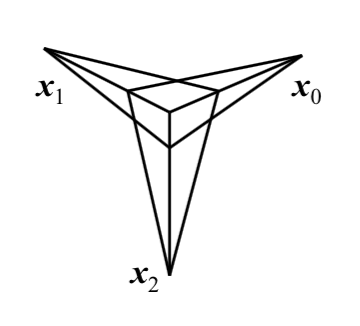
\includegraphics[width=0.4\textwidth]{figures/vanishing_points.png}
\end{center}
\caption{Visualisation of how the edges of a cuboid give rise to three orthogonal vanishing points.} % TODO hur referera? Tagen från szeliski s. 330
\label{fig:vanishing_points}
\end{figure}

The online configuration uses vanishing point calibration.
It is ideal to use vanishing point calibration for this particular problem since every cuboid package has three orthogonal sets of parallel lines which result in three orthogonal vanishing points.
Additionally, the known homography between the image plane and the top-plane of the package can be used to improve the estimate of $K$.

When the $K$ is known, the camera pose can be estimated as described in \ref{camera-pose}, using the four image-world point correspondences given by the reference object.
The method EPnP was chosen initially, but much better results were achieved with a regular, iterative approach. % TODO refer opencv?

Once the camera pose is obtained, equation \ref{eq:projection1} can be used, which means that any point in the world can be projected to a point in the image.
However, the reverse mapping is sought, i.e. the position of the package the world of the image coordinates of the bottom corners of the package, i.e. the reverse mapping.
This is generally not possible to do, unless something is known about the geometry of the scene.
Luckily, it is known that the lower corners share $X$, and $Y$ coordinates with a top corner, which position is already known.
The image coordinates $(u,v)$ of a lower corner, and the world coordinates $(X,Y)$ of the corresponding upper corner can then be used to solve for the $Z$ coordinate of the lower corner. 
Equation \ref{eq:projection3} can be transformed to the following over-defined system:
\begin{equation} \label{eq:constrained-projection}
\begin{pmatrix} up_{33}-p_{13} \\ vp_{33}-p_{23} \end{pmatrix} Z = 
\begin{pmatrix}
X(p_{11}-up_{31}) + Y(p_{12}-up_{32})+p_{14}-u \\
X(p_{21}-vp_{31}) + Y(p_{22}-vp_{32})+p_{24}-v
\end{pmatrix}
\end{equation}
This is solved as a least-squares problem using Single Value Decomposition (SVD).
Since two pairs of upper-lower corners which share $X$ and $Y$ coordinates are known, two least-squares solutions of $Z$ can be obtained.
The solution with the smallest error is chosen as $Z$.

\section{Evaluation}
To evaluate the performance of the detection and measuring algorithms two datasets were gathered.
One training dataset, used to optimise the many constants used by the algorithms, and one test dataset. % TODO how many constants? How is optimisation done?
The training dataset consisted of 50 images of five different packages.
The test dataset consisted of 225 images of five different packages.
The packages in the test dataset are shown in figure \ref{fig:packages} and their dimensions are shown in table \ref{table:package_dimensions}.

\begin{table}
\centering
\begin{tabular}{@{} *4c @{}}
\toprule
\multirow{2}{*}{Package$~\#$} & \multicolumn{3}{c}{Dimensions ($mm$)}\\ 
\cmidrule(r){2-4}
 & Length & Width & Height \\
 \midrule
 1 & 580 & 350 & 405 \\ 
 2 & 260 & 191 & 177 \\
 3 & 385 & 295 & 225 \\
 4 & 580 & 360 & 670 \\
 5 & 383 & 280 & 590 \\
\bottomrule
 \end{tabular}
 \caption{Dimensions in millimetres of packages in test dataset.}
\label{table:package_dimensions}
\end{table}

\begin{figure}
\begin{center}

\includegraphics[width=0.4\textwidth]{figures/placeholder.png}
\end{center}
\caption{The packages in the test dataset.}
\label{fig:packages}
\end{figure}

The test dataset was constructed systematically with images observing the packages from different poses. % TODO correct sentence?
Three parameters were alternated: 
\begin{itemize}
	\item Distance to the centre of the package. 
			The considered distances were 1, 1.5, and 2 metres.
	\item Height above the ground. 
			The considered heights were 0.9, 1.2, and 1.5 metres for the first three packages, and 1.2, 1.5, and 1.8 metres for the latter two.
			The reason for the division is that the high height of the two latter packages made the viewing angle unreasonable when viewing them from 0.9 metres above ground, so the lowest height was removed, and a higher one added.
	\item Horizontal viewing angle. 
			Five different angles were used.
			Two were frontal views of the package, in which only two faces of the package could be observed. One of the longer side, and one of the shorter side.
			One image was taken between the two sides, with a $45^\circ$ angle to both sides.
			The last two images view the package with a sharp angle, about $15^\circ$ to the long or short side, respectively.
			A sample image from each position is shown in figure \label{fig:positions}.
\end{itemize}

\begin{figure}
\begin{center}

\includegraphics[width=0.4\textwidth]{figures/placeholder.png}
\end{center}
\caption{Figure showing the different horizontal viewing positions.}
\label{fig:positions}
\end{figure}

All combinations of distances, heights, and horizontal angles resulted in 45 images per package.

\subsection{Benchmarking}
A benchmarking program was constructed in order to measure the performance of the algorithms in the different cases.
The program ran the algorithms on each image, while gathering information about the success rates and accuracy.
The detection algorithm and measuring algorithm were tested both independently, and together, to show the performance of the individual pieces and of the whole system. 

The detection algorithm was tested by comparing the outputted corner points against ground truth locations of the reference object and package corners, which had been manually marked in each image.
The ability to detect the reference object, the package, and both in the same image, was tested.

The measuring algorithm was tested by using the ground truth locations as input, and comparing the resulting measurements against the ground truth dimensions of the package.
Both calibration methods, online vanishing point calibration, and offline calibration with Zhang's method, were tested.

The overall ability of the system was tested by running the whole algorithm and comparing the result with the ground truth dimensions of the package. 

%To simplify evaluation a test file (in JSON format) with information about each image was created.
%Each file contained information about which package was displayed in the image, the path to the image, the distance, height, and horizontal angle to the package, the dimensions of the package, and the locations of reference object and package corners in the image, which had been marked manually.



\subsection{Online testing}
A simple proof of concept Android application was made for online testing on the phone.
This was used to assert that it is feasible to run the algorithm on a smartphone.
Its purpose was also to determine if running the detection algorithm in real-time was an option.

The app simply displays the camera feed and continuously feeds new frames to the measuring algorithm.
When the package or reference object is successfully detected, an overlay is drawn to outline their position on the screen.
If both the package and reference are found in the same frame, the dimensions of the package are calculated, and each dimension is drawn next to the appropriate edge.
The processing time for each frame is also displayed.

The device used to run the test app is a Samsung Galaxy S6 Edge.
The S6 Edge was chosen because it currently tops benchmarks and tests, both regarding processing power and photo quality \cite{phone_performance_benchmark}\cite{phone_camera_benchmark}.
The S6 Edge was also used to capture the test images used for offline testing.










